% This file was created by matlab2tikz.
%
%The latest updates can be retrieved from
%  http://www.mathworks.com/matlabcentral/fileexchange/22022-matlab2tikz-matlab2tikz
%where you can also make suggestions and rate matlab2tikz.
%
\definecolor{mycolor1}{rgb}{0.00000,0.44700,0.74100}%
\definecolor{mycolor2}{rgb}{0.85000,0.32500,0.09800}%
\definecolor{mycolor3}{rgb}{0.92900,0.69400,0.12500}%
%
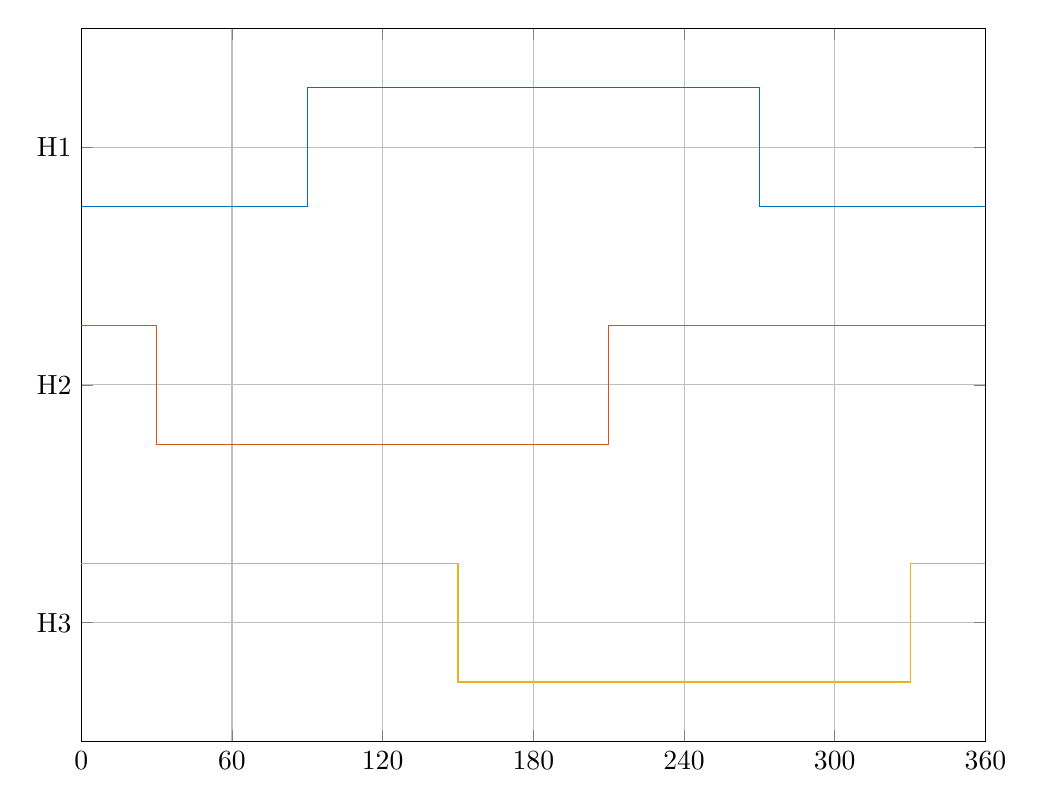
\begin{tikzpicture}

\begin{axis}[%
width=4.521in,
height=3.566in,
at={(0.758in,0.481in)},
scale only axis,
xmin=0,
xmax=360,
xtick={  0,  60, 120, 180, 240, 300, 360},
ymin=-1,
ymax=11,
ytick={1,5,9},
yticklabels={{H3},{H2},{H1}},
axis background/.style={fill=white},
xmajorgrids,
ymajorgrids
]
\addplot[const plot, color=mycolor1, forget plot] table[row sep=crcr] {%
0	8\\
30	8\\
60	8\\
90	10\\
120	10\\
150	10\\
180	10\\
210	10\\
240	10\\
270	8\\
300	8\\
330	8\\
360	8\\
};
\addplot[const plot, color=mycolor2, forget plot] table[row sep=crcr] {%
0	6\\
30	4\\
60	4\\
90	4\\
120	4\\
150	4\\
180	4\\
210	6\\
240	6\\
270	6\\
300	6\\
330	6\\
360	6\\
};
\addplot[const plot, color=mycolor3, forget plot] table[row sep=crcr] {%
0	2\\
30	2\\
60	2\\
90	2\\
120	2\\
150	0\\
180	0\\
210	0\\
240	0\\
270	0\\
300	0\\
330	2\\
360	2\\
};
\end{axis}
\end{tikzpicture}%